\documentclass[titlepage,12pt]{article}
\renewcommand{\figurename}{Рис.}
\usepackage[T2A]{fontenc}
\usepackage[cp1251]{inputenc}  
\usepackage{amsmath}
\usepackage{amssymb}
\usepackage{graphicx}

\oddsidemargin = 0.6cm
\textwidth = 16cm
\textheight = 21cm
\headheight = 0cm
\sloppy

\author{Кочуркин Иван Алексеевич\\ Группа ИУ7-92 \\ Вариант \textnumero 11}
\title{Отчёт по лабораторной работе \textnumero 2 \\по курсу\\ Методы вычислений}
\date{2011 г.}

\newcommand{\D}[2]{\frac{\partial #1}{\partial #2}}
\newcommand{\DD}[2]{\frac{\partial^2 #1}{\partial #2^2}}

\begin{document}

\maketitle
\setcounter{page}{2}
\newpage

\section{Постановка задачи}
Найти функцию $u(x,t)$, описывающую поперечные малые колебания однородной струны длины $1$, концы которой движутся по заданным
законам. Значение $u(x,t)$ задает величину отклонения точки струны с координатой $x$ в момент времени $t$ от положения равновесия. Движение левого конца струны $(x = 0)$ определяется законом $u(0,t) = \mu(t)$, правого ($x = l)$ - законом $u(l,t) = \nu(t)$. Начальное положение струны $u(x,0) = \phi(x)$, начальная скорость $u_t(x,0) = \psi(x)$.
Уравнение, описывающее колебания струны: $u_{tt} = a^2 u_{xx}$.

\begin{eqnarray}
u_{tt} &=& a^2 u_{xx}, \\
u(0, t) &=& \mu(t), \\
u(l, t) &=& \nu(t), \\
u(x, 0) &=& \phi(x), \\
u_t(x, 0) &=& \psi(x). \\
\end{eqnarray}

Исходные данные:

\[
\left\{
\begin{array}{rl}
\varphi(x) &= (1-x)cos(\frac {\pi x} {2}), \\
\psi(x) &= 2x+1, \\
\mu(t) &= 1+t-t^2, \\
\nu(t) &= 0 \\
a &= 1, \\
l &= 1. \\
\end{array}
\right.
\]

\section{Решение}
Сеточный метод, основанный на замене в дифференциальном уравнении производных конечными разностями, называют методом конечный разностей, а сеточную схему такого метода разностной схемой. Разностная схема: для численного решения данного уравнения использовалась явная разностная схема “крест”.

Для решения задачи сеточным методом выберем равномерную прямоугольную сетку с узлами $(x_i,t_j), i=\overline{0,N}, j=\overline{0,M}, x_i=ih, t_j=j\tau, h=\frac{l}N, \tau=\frac{T}M $. Частные производные заменяем соответствующими разностями. В результате дифференциальное уравнение сведется к разностномым уравнениям:
\begin{equation}
\frac{u^{j+1}_i - 2 u^j_i + u^{j-1}_i}{\tau^2} = a^2 \frac{u^j_{i-1} - 2u^j_i + u^j_{i+1}}{h^2}\\
\end{equation}
начальное условие $u(x, 0) = \phi(x) $ заменяется разностным соотношением:
\begin{equation}
\frac{u_i^1-u_i^0}{\tau}=\psi_i, i=\overline{1,N-1}.\\
\end{equation}
Другое начальное условие и граничные условия в разностной задаче реализуются точно:
\begin{equation}
u_i^0=\phi_i, i=\overline{0,N}; u_0^j=\mu^j, u_N^j=\nu^j, j=\overline{1,M}
\end{equation}

По начальному положению струны определяется значение сеточной функции на нулевом слое. По начальным скоростям определяются значения сеточной функции на первом слое. Наконец, по разностному уравнению можно вычислисть значения сеточной функции во внутренних узлах (j+1)-го слоя по уже известным значениям двух предыдущих слоев. Значения в граничных узлах (j+1)-го слоя находятся из граничных условий.

\subsection{Устойчивость}

Для обеспечения устойчивости данной разностной схемы между шагами по длине и по времени должно выполняться соотношение:

\begin{equation}
\frac{a^2 \tau^2}{h^2} \leq 1
\end{equation}

\subsection{Аппроксимация}
Замена дифференциального уравнения разностным происходит с порядком аппроксимации $O(\tau^2 + h^2)$. Для аппроксимации начальных скоростей использовалось соотношение, обеспечивающее порядок аппроксимации $O(\tau)$. Левое и правое граничные условия в точности соответствуют условию непрерывной задачи.

\subsection{Определение ошибки}
Для определения ошибки воспользуемся формулой Рунге 
$$
z^I \approx \frac{|u^I - u^{II}|}{r^2-1}
$$
один раз, приняв $r=2$. При этом используется обычная сетка $\omega^I$ с шагами $\tau$ и $h$ и сгущённая сетка $\omega^{II}$.Шаги у сгущённой сетки $\omega^{II}$ будут соответственно $\tau / r$ и $h/r$.\par
Результаты: максимальная погрешность  $z^I_{max} = 0.008118$, среднее значение погрешности $\overline{z^I} = 0.000592$.

\newpage
\subsection{График}
\begin{figure}[h]
\centering
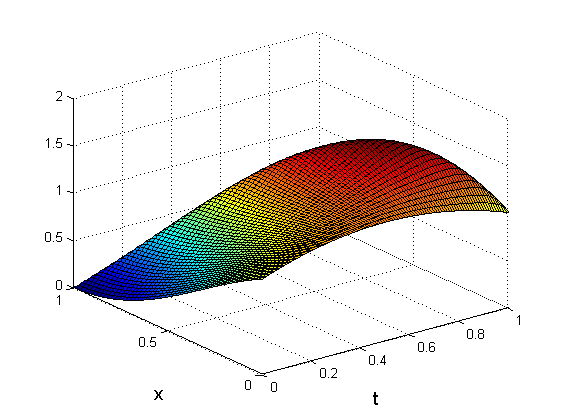
\includegraphics[width = 16cm]{Screen}
\caption{Колебания струны}
\label{fig:res}	
\end{figure}

\end{document}
